\documentclass[RNAAS]{aastex631}

\usepackage{natbib}
\usepackage{graphicx}
\usepackage{amsmath}

\shorttitle{Anomalous SEDs in CEERS DR1}
\shortauthors{Shasti-Nazem et al.}

\begin{document}

\title{A Search for Anomalous Spectral Energy Distributions in CEERS DR1: An
Open-Source JWST Anomaly Detection Pipeline}

\author[0009-0006-7506-5070]{Armeen Shasti-Nazem}
\affiliation{Department of Astronomy, University of Washington, Seattle, WA
98195, USA}
\email{aasha@uw.edu}
% Additional co-authors (e.g., faculty advisor) to be added before submission.

\section{}

JWST NIRCam surveys now provide photometric catalogs large enough to search
systematically for galaxies whose SEDs are not well described by standard
stellar-population templates. We present an open-source pipeline that fits
photo-$z$'s and best-fit template SEDs with EAZY \citep{Brammer2008}, scores
per-band residuals with an Isolation Forest + UMAP/DBSCAN ensemble, and
cross-matches flagged sources against known contaminants, applied to the
CEERS Data Release 1.0 catalog \citep{Cox2025}.

Of 87,345 CEERS DR1.0 sources ingested, redshift-window
($0.5 \le z_{\rm phot} \le 10$) and coverage cuts retain 68,839 for EAZY
fitting; its fit-failure sentinel ($\chi^2_{\rm EAZY}<0$) excludes 2,900
(4.2\%) as non-converged artifacts, leaving a clean sample of 65,939
sources, of which the top 2\% (1,319) are flagged as anomalous.
Cross-matching against Milliquas v8 \citep{Flesch2023} within 1\farcs5 finds
only 5 matches (0.38\%): known AGN explain a negligible fraction of the
flagged population.

Figure~\ref{fig:zrate} bins the flagged rate in $\Delta z=0.5$ shells; an
OLS fit finds no significant redshift trend ($p=0.32$). Following the
conservative Bayesian framework of \citet{Wright2014} and
\citet{LingamLoeb2019}, we adopt a prior $P(H_1)=10^{-8}$ per source and the
flagged sample's unexplained fraction as $P(\mathrm{unexplained}\mid H_0)$;
the posterior that an unexplained flagged source reflects non-standard
physics is $P(H_1\mid\mathrm{unexplained})\approx1.12\times10^{-8}$, almost
unchanged from the prior, since being unexplained is the norm here --- a
reproducible upper limit on non-standard astrophysics at current CEERS
depth.

\begin{figure}[h]
\centering
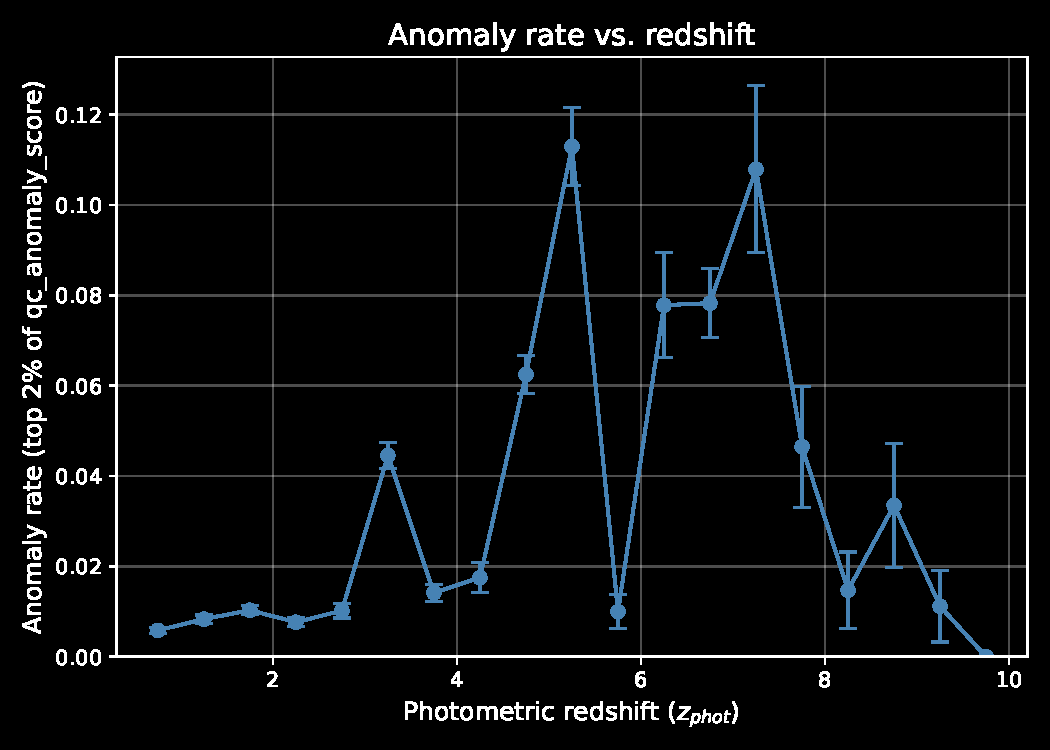
\includegraphics[width=0.15\linewidth]{../figures/anomaly_rate_vs_redshift.pdf}
\caption{Flagged rate vs.\ $z$, clean sample ($N=65{,}939$), Poisson error
bars; rates span $\sim$0--11\%; $p=0.32$.}
\label{fig:zrate}
\end{figure}

Code: \url{https://github.com/Menrae/jwst-sed-anomaly}. \software{astropy,
eazy-py \citep{Brammer2008}, scikit-learn, umap-learn, xarray}

\vspace{-1.1\baselineskip}
\bibliographystyle{aasjournal}
\bibliography{references}

\end{document}
